
\section{Guidelines}

Please write a short paper about your project. There are no strict length limits, but please write \textbf{at least two pages in the layout of this template} (including figures, excluding references and code listings). Please structure your paper in a scientific way, and include your references and your code. There are \LaTeX packages you can use to preserve the indentation of your code, e.g. the \texttt{listings} package which is demonstrated in the Appendix~\ref{app:codes}.

This sample document makes use of of REV\TeX~4.2, therefore you will need to install it to be able to compile this document yourself. Further information can be found in the REV\TeX~4.2
documentation included in the distribution or available at
\url{http://journals.aps.org/revtex/}.


\subsection{Example citations}
By default, citations are numerical\cite{epr}, some more citations~\cite{feyn54,Bire82,Berman1983,witten2001,Davies1998}. 

\subsection{Exampe figure}
Including and referring to figures is as usual, see for instance Fig.~\ref{fig:example}
\begin{figure}
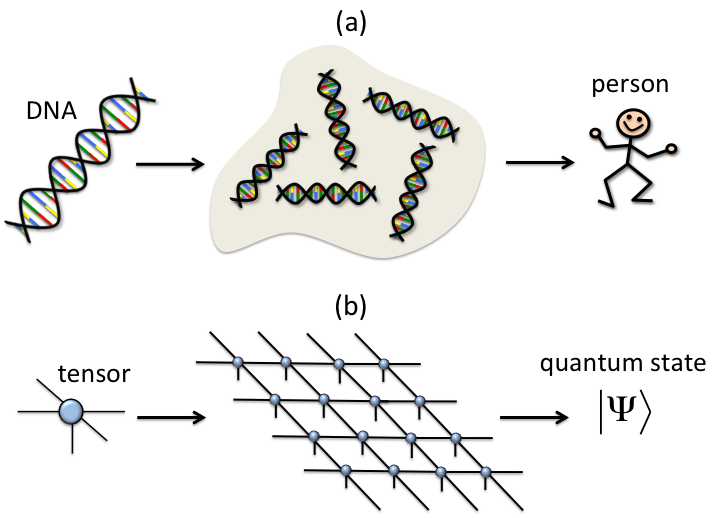
\includegraphics[width=0.99\linewidth]{cartoon.png}
\caption{Example of a figure from Ref.~\cite{Orus2013}.}
\label{fig:example}
\end{figure}